   \begin{figure}[h]
        \centering
		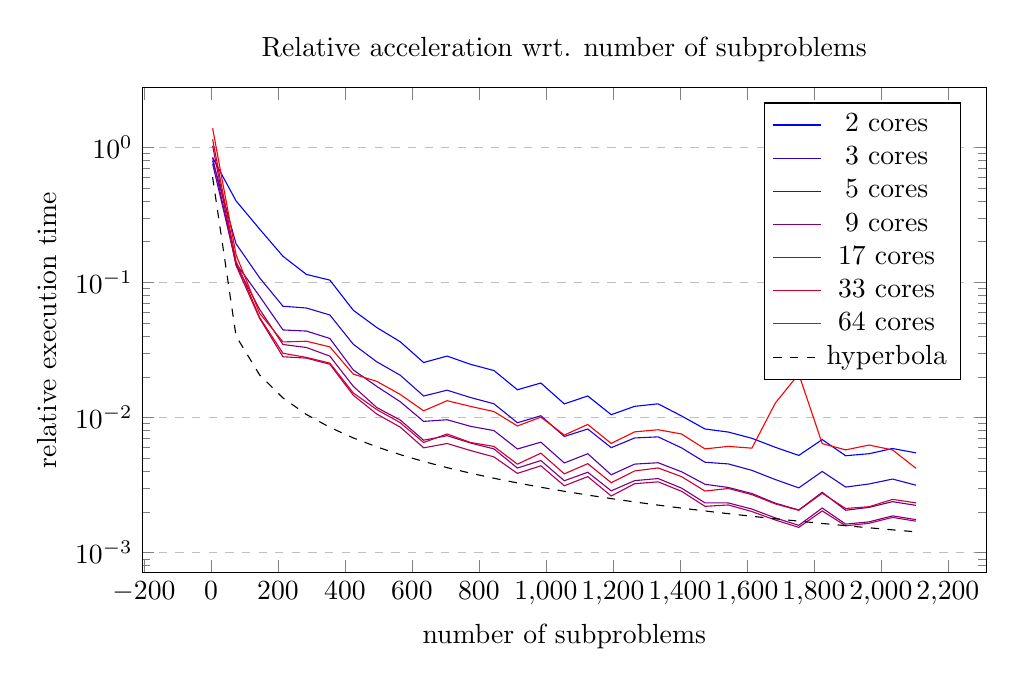
\begin{tikzpicture}
		\begin{axis}[
			title={Relative acceleration wrt. number of subproblems},
			xlabel={number of subproblems},
			ylabel={relative execution time},
			%xmin=0, xmax=0.25,
			%ymin=10.00, ymax=100000.00,
			ymode=log,
			%xmode=log,
			%xtick={0,0.05,0.1,0.15,0.2,0.25},
			%ytick={0,20,40,60,80,100},
			%yticklabel=$\pgfmathprintnumber{\tick}\%$,
			legend pos=north east,
			ymajorgrids=true,
			grid style=dashed,
			xticklabel style={/pgf/number format/fixed},
			width = 350,
			height = 220
		]




\addplot[color=red!0.0!blue,line width=0.4pt] coordinates {
(5,0.8363703260509081)(75,0.40044086669564954)(145,0.24820760445286044)(215,0.15586154433903676)(285,0.11441574489877396)(355,0.10383228199616126)(425,0.062112244462297336)(495,0.04631987498640051)(565,0.0363514389443031)(635,0.0255062395908254)(705,0.028461983857429193)(775,0.024729523125231637)(845,0.02224756104517527)(915,0.016031056959308215)(985,0.017990965806449793)(1055,0.012602624715768295)(1125,0.014428008140009687)(1195,0.010483218052462122)(1265,0.012090345845853636)(1335,0.012617655143597912)(1405,0.010260395984662996)(1475,0.00821915969199854)(1545,0.007797760326512107)(1615,0.007015986107255104)(1685,0.006015559914820198)(1755,0.005238103290395365)(1825,0.006863269191829858)(1895,0.005212129656505115)(1965,0.005394250241223485)(2035,0.005892540631817077)(2105,0.005470470118470802)
}node[pos=0.8](endofplotsquare){} ;
\addlegendentry{2 cores}
\addplot[color=red!16.666666666666668!blue,line width=0.4pt] coordinates {
(5,0.7953947640462143)(75,0.19287219486951168)(145,0.10821465405457484)(215,0.06655933633194881)(285,0.06455734436647677)(355,0.05731206548874832)(425,0.0348103366827173)(495,0.02582226849746521)(565,0.020555985130909643)(635,0.014414085069604093)(705,0.015914041554104696)(775,0.01404563934603624)(845,0.012622724691626362)(915,0.00914084020222177)(985,0.01030137267781949)(1055,0.007236220870675304)(1125,0.008216274992029135)(1195,0.00597728023540709)(1265,0.0070535371403745335)(1335,0.007186896657302999)(1405,0.005957848712307183)(1475,0.004664177373220047)(1545,0.004531664358657725)(1615,0.004062888962836021)(1685,0.003472003348871099)(1755,0.003014331883154194)(1825,0.003989341538922921)(1895,0.0030551923392005942)(1965,0.0032216065883479707)(2035,0.0035026558761778624)(2105,0.00315456432254383)
}node[pos=0.8](endofplotsquare){} ;
\addlegendentry{3 cores}
\addplot[color=red!33.333333333333336!blue,line width=0.4pt] coordinates {
(5,0.7540799612489124)(75,0.13770773845147158)(145,0.07903118735302324)(215,0.0444292876122649)(285,0.04359841132583865)(355,0.03843108751108544)(425,0.022476245693874835)(495,0.016992134208814662)(565,0.013085171580030565)(635,0.009354873212661784)(705,0.009623132156813024)(775,0.008601600810769768)(845,0.007997350837381617)(915,0.005844809497154642)(985,0.006566702190397072)(1055,0.0046066955464967385)(1125,0.005391459880088773)(1195,0.003765944493922464)(1265,0.004517972989232357)(1335,0.004625354886416106)(1405,0.003967271630504892)(1475,0.003204556537457041)(1545,0.003033559290311071)(1615,0.002736811668500518)(1685,0.0023219705479595233)(1755,0.0020689990640417135)(1825,0.0027955377403811573)(1895,0.002059099664076773)(1965,0.002161659972390088)(2035,0.0023835551937098024)(2105,0.0022366735124972883)
}node[pos=0.8](endofplotsquare){} ;
\addlegendentry{5 cores}
\addplot[color=red!50.0!blue,line width=0.4pt] coordinates {
(5,0.8395180080320743)(75,0.13518033229705892)(145,0.06329495573875105)(215,0.03467498095786615)(285,0.032946276058190636)(355,0.02843740849447381)(425,0.01700059475426545)(495,0.01185082078331524)(565,0.009583217651849624)(635,0.0067879373357470785)(705,0.00733279588264961)(775,0.006473730136613454)(845,0.00585275388825431)(915,0.004223941423046687)(985,0.0048023948235786365)(1055,0.0034030299592173706)(1125,0.003932382641530949)(1195,0.0028652830044705252)(1265,0.003409755894449815)(1335,0.003533730715612736)(1405,0.003001564873126131)(1475,0.0023343136294482034)(1545,0.002331287468822943)(1615,0.002099444456355938)(1685,0.0018067291136231742)(1755,0.0015921906675146404)(1825,0.002138097873277723)(1895,0.0016254754718868349)(1965,0.0016898415459182174)(2035,0.0018712422685091005)(2105,0.0017544596847386673)
}node[pos=0.8](endofplotsquare){} ;
\addlegendentry{9 cores}
\addplot[color=red!66.66666666666667!blue,line width=0.4pt] coordinates {
(5,1.0233671083266738)(75,0.13298582581574836)(145,0.054342141287111095)(215,0.028136617662919666)(285,0.0274850117836712)(355,0.024767735467616722)(425,0.014603392440664225)(495,0.01060627134337961)(565,0.008489780577146392)(635,0.005960846427571119)(705,0.006419783187656039)(775,0.005693731627707895)(845,0.005107422343337776)(915,0.003857476739178135)(985,0.004391044049971209)(1055,0.0031239152675193596)(1125,0.0036507550214886614)(1195,0.0026247982449260168)(1265,0.003233826478061956)(1335,0.0033403745852336394)(1405,0.0028430792367325646)(1475,0.002200627944362014)(1545,0.0022523276938355174)(1615,0.002013942986585552)(1685,0.0017432388265270233)(1755,0.0015377756992326164)(1825,0.0020356102833054817)(1895,0.0015788129786271285)(1965,0.0016499736740357815)(2035,0.001822449738409042)(2105,0.0017085385916049166)
}node[pos=0.8](endofplotsquare){} ;
\addlegendentry{17 cores}
\addplot[color=red!83.33333333333333!blue,line width=0.4pt] coordinates {
(5,1.1430591924550146)(75,0.1430227631420044)(145,0.0550902628411104)(215,0.029860641277366737)(285,0.027825714476219225)(355,0.025254507640047268)(425,0.015181667878617168)(495,0.011448534033175722)(565,0.00915695381741731)(635,0.0065301049757312294)(705,0.007550217807928795)(775,0.006531482865975962)(845,0.0061084692678245595)(915,0.004514001544709272)(985,0.005442886204953784)(1055,0.0038276532255329407)(1125,0.004553502202237839)(1195,0.0032922630420942297)(1265,0.004022898124369985)(1335,0.004232557187196659)(1405,0.003650674441859657)(1475,0.002855195221820208)(1545,0.0029828610389978022)(1615,0.002686401608577915)(1685,0.0022927407726168027)(1755,0.0020568970810727625)(1825,0.0027495482073485065)(1895,0.002122191389302815)(1965,0.0021869364529382984)(2035,0.0024771185156596577)(2105,0.002335438636016641)
}node[pos=0.8](endofplotsquare){} ;
\addlegendentry{33 cores}
\addplot[color=red!100.0!blue,line width=0.4pt] coordinates {
(5,1.3804728949138354)(75,0.15989108763659018)(145,0.05923250293374861)(215,0.03623345150554006)(285,0.0366491697816772)(355,0.033302831517728865)(425,0.020934522465703542)(495,0.01850792801621138)(565,0.014818050848156503)(635,0.01120213017824374)(705,0.013307029888745294)(775,0.012078063979757607)(845,0.011056552004666573)(915,0.008652946816065623)(985,0.010058157334588409)(1055,0.007411647218094335)(1125,0.008876128923162509)(1195,0.006425619803304469)(1265,0.007824727583313294)(1335,0.008115708281487758)(1405,0.007548032452182414)(1475,0.005855031785751925)(1545,0.006111780178658547)(1615,0.0059283175789550694)(1685,0.012789253519400294)(1755,0.020957095312401513)(1825,0.0064057552276834415)(1895,0.005760009494321792)(1965,0.006250122294819795)(2035,0.005750178328994417)(2105,0.004205274975490067)
}node[pos=0.8](endofplotsquare){} ;
\addlegendentry{64 cores}
\addplot[color=black,line width=0.4pt,dashed] coordinates {
(5,0.6)(75,0.04)(145,0.020689655172413793)(215,0.013953488372093023)(285,0.010526315789473684)(355,0.008450704225352112)(425,0.007058823529411765)(495,0.006060606060606061)(565,0.005309734513274336)(635,0.004724409448818898)(705,0.00425531914893617)(775,0.003870967741935484)(845,0.0035502958579881655)(915,0.003278688524590164)(985,0.003045685279187817)(1055,0.002843601895734597)(1125,0.0026666666666666666)(1195,0.002510460251046025)(1265,0.0023715415019762848)(1335,0.0022471910112359553)(1405,0.002135231316725979)(1475,0.002033898305084746)(1545,0.001941747572815534)(1615,0.0018575851393188853)(1685,0.0017804154302670622)(1755,0.0017094017094017094)(1825,0.0016438356164383563)(1895,0.0015831134564643799)(1965,0.0015267175572519084)(2035,0.0014742014742014742)(2105,0.0014251781472684087)
}node[pos=0.8](endofplotsquare){} ;
\addlegendentry{hyperbola}

		\end{axis}
		\end{tikzpicture}
		%\vspace{-18pt}
		\caption[Runtime relative acceleration of paralell small-hard problems]{Runtime relative acceleration on paralell small-hard subproblems, relative to Tinisat time, with hyperbolic trendline, for different numbers of cores and subproblems}
		\label{fig:performance_graph1}
    \end{figure}
